%!TEX root = ../thesis.tex

\section{Blue face subdivision}
\label{s:subdiv}


At this point we have a vertically one-sided graph (due to Lemma \ref{lm:topfan:oneSidedREL}) without large topfans except possibly for the locations provided in Lemma \ref{lm:topfan:remainingTopfans}.

\paragraph{Outline}
In this stage we are going to recolor edges in all blue faces to make all of them $d+1$-sided. We will start at the bottommost face in the creation order (which we will have to recalcualte after the topfanflips, but every REL has one). And we will recolor some if it's edges if a blue face that is to large will appear.

We then mark the edges on the top boundary path of this face above the recolored edges as \emph{loaded}. This means that we will try to not flip above these edges in future iterations of the algorithm.

Then we continue with the next face in the order we just calcualted.

\paragraph{Order of faces}
TODO

\paragraph{Loads}
TODO what is a load, puttting trough loads


\paragraph{Step requirements}
We flip edges in each face, taking into account loads on the bottom fence. Such that

\begin{enumerate}
  \item We never load the edge next to a split/merge
  \item We never load two adjacent edges
\end{enumerate}

It's important to note that we put trough edge loads on splits and merges

Because we do this we can also say the following

\begin{lemma}
  \label{lm:}
  On the bottom boundary path of every face we never find two subsequent loaded edges. Even when we put trough loads on splits and merges.
\end{lemma}
\begin{proof}
  A single face would never load two subsequent edges. Hence the only way to get two subsequent loaded edges is using different faces and thus splits and merges.

  However due to the built-in safety of never flipping next to a split/merge we never get subsequent    loaded edges.
  \fxnote{Might add a figure}
\end{proof}


\subsection{Faces without large topfans}
Let us first consider the base case: no failed top fan flips and thus no large topfans

\begin{lemma}
  \label{lm:}
  We can subdivide any blue face without large topfans into 7-sided chunks while obeying the load rules above.
  That is: We have at most one toploaded edge. On the bottom we never have two subsequent loaded edges. All topfans are of size 2.
  \fxnote{We can make this Lemma WAY tighter if all topfans are of size exactly 2}
\end{lemma}

\begin{proof}
  A worst case example is given in Figure \ref{fig:subdiv:worstCase}.

  \begin{figure}[h]
    \centering
    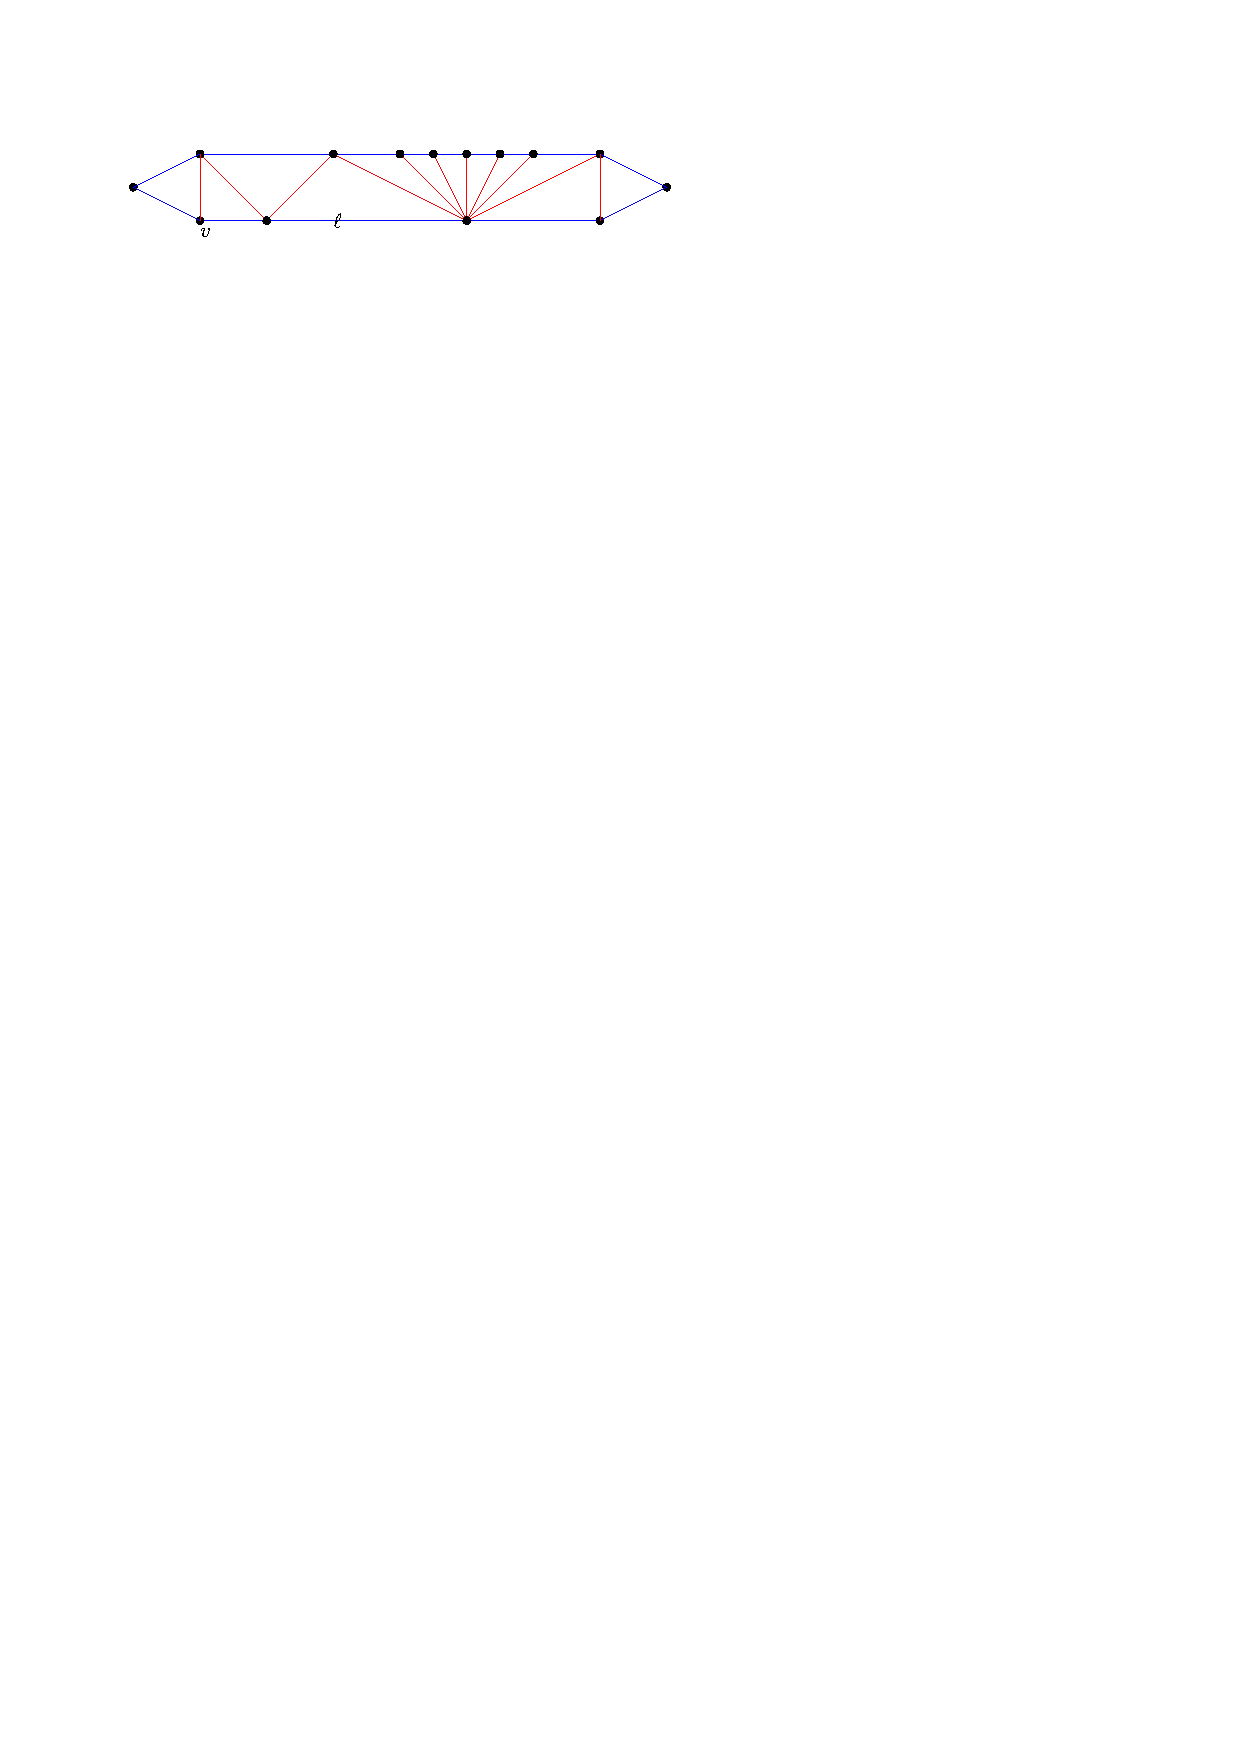
\includegraphics[scale=1]{blueFaceSubdivision/img/worstCase}
    \caption{A worst case blue face. We don't flip any edge in this face.}
    \label{fig:subdiv:worstCase}
  \end{figure}
  \fxwarning{TODO update figure}

  Note that we can flip above each edge in the bottom boundary path.

  We will look at the vertex on the bottom fence that's adjacent to the freshly flipped edge,  or if we haven't flipped an edge yet the vertex next to the split (and we will call it $v$). The following are then the rules for flipping above the edges following $v$.
  \begin{enumerate}
    \item We don't flip above the first edge.
    \item We flip above the second edge if it's unloaded.
    \item Otherwise we flip above the third edge.
    \item We never flip next to the merge the merge
  \end{enumerate}

  When flipping above a edge we always flip the right edge.

The first edge give us the required separation of loaded edges along the top boundary path. The other items make sure we obey the other rules in a straightforward manner.

The worst case is given by a combination of the last two items. We would in that case want to flip above the third edge. But we don't because the next edge is the merge. This gives at worst 5 edges along the whole bottom boundary path and hance a 4-sided face.



See Figure \ref{fig:subdiv:sampleExecution} for an example of an execution of this algorithm.
\fxwarning{TODO update figure}

\begin{figure}[h]
  \centering
  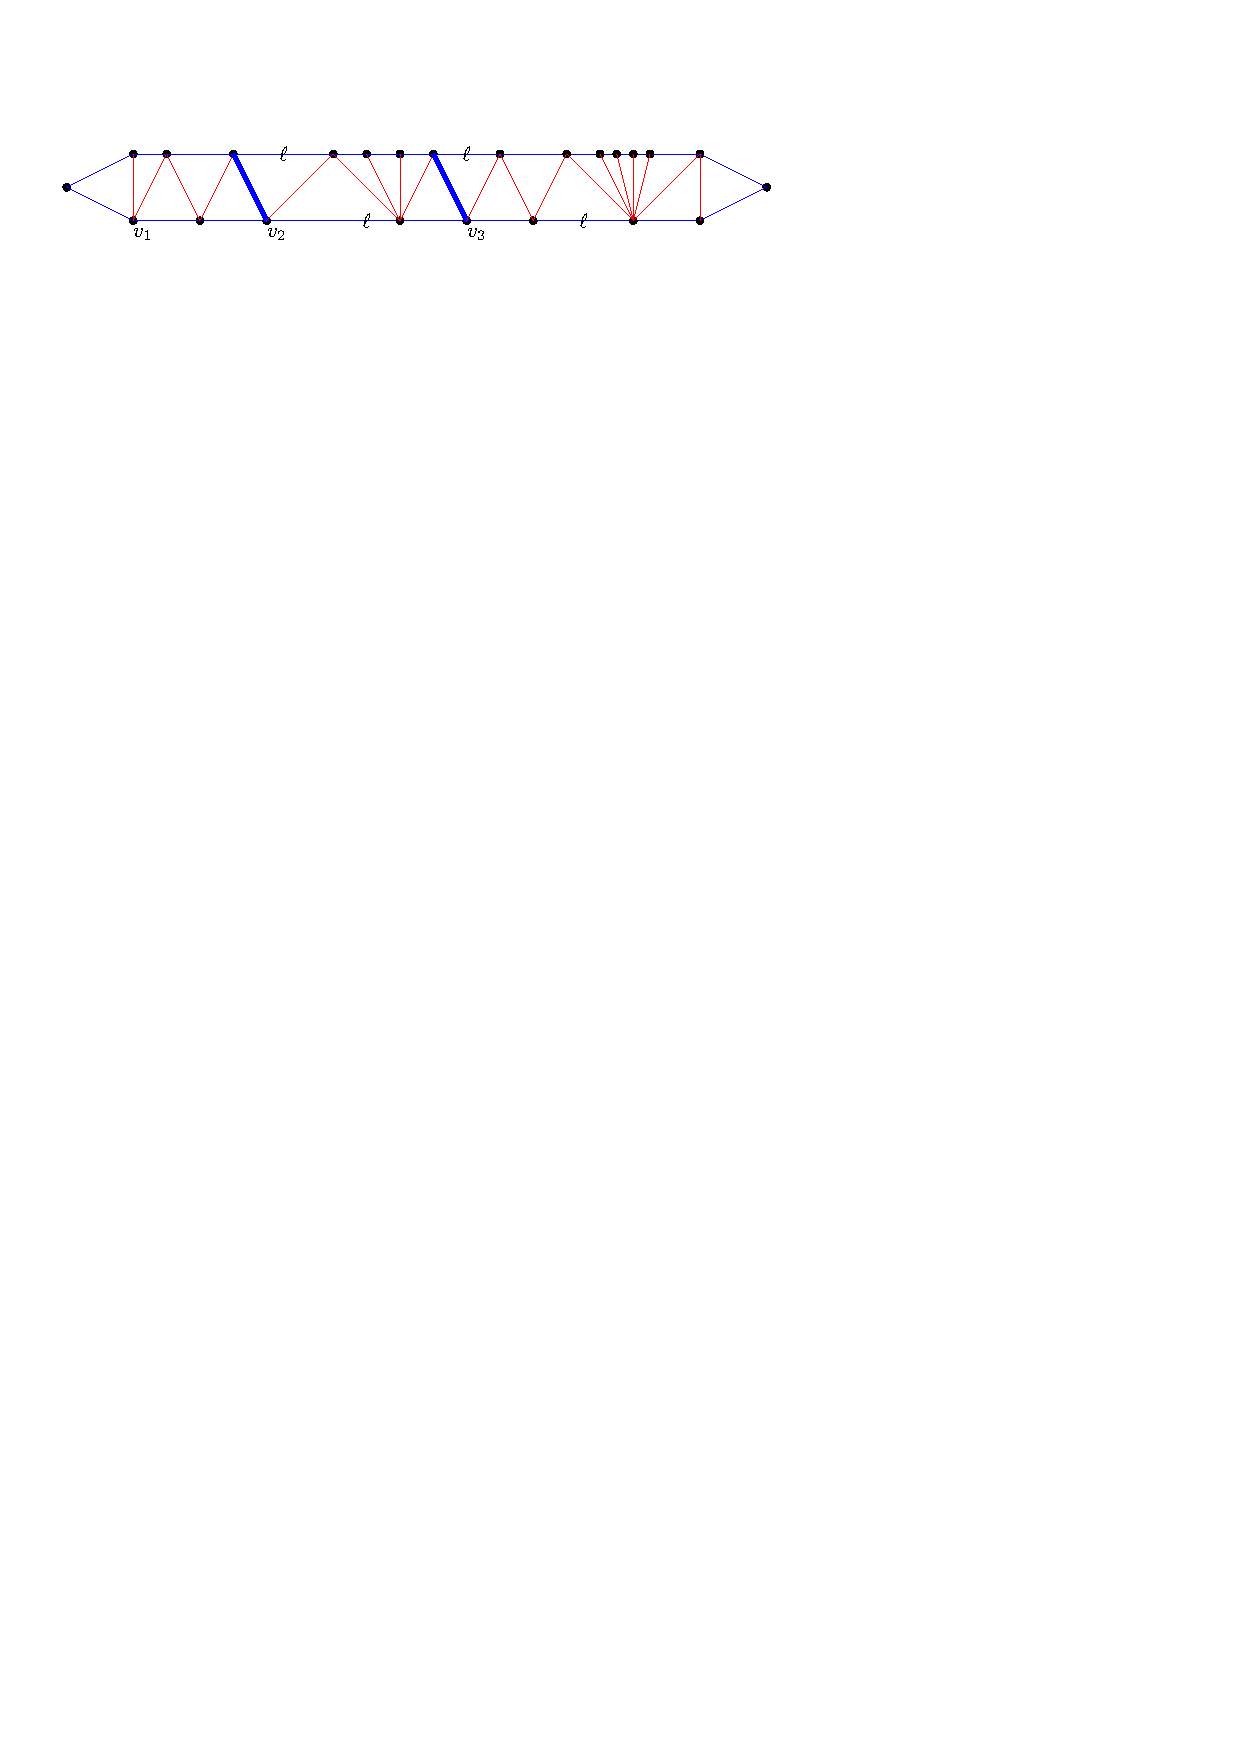
\includegraphics[scale=1]{blueFaceSubdivision/img/sampleExecution}
  \caption{Sample execution of the algorithm}
  \label{fig:subdiv:sampleExecution}
\end{figure}

\end{proof}


\subsection{Face starting with a large topfan}
The same algorithm finds us an edge keeping this face as a $ d - 3 +4 = d+1$ face.
\fxwarning{TODO write this}

\subsection{Face encountering a larger topfan}
If we have a large topfan in the middle of the face then above the left outer edge of this topfan we can't have another topfan that failed to flip its left outer edges.
It can't have been due to split on the first vertex because that would imply a chord trough the current large topfan \fxwarning{TODO make this a lemma in the right place}

It can't have been due to $\pS$-adjecency. Because the first edge of such a flip is adjacent to $\pS$ and thus can't be above the middle of some face.

The other topfans are at the start of a face, so their left edge is flipped. So in that case we evaded loaded edges.

This leads to the following rule: we flip the first edge of a topfan even above a loaded edge.
\fxwarning{TODO write this}


\subsection{General conclusion}
\begin{lemma}
  \label{lm:}
  We have a d+1-sided REL
\end{lemma}

\begin{proof}
  By construction a blue faces are $d+1$-sided. We have  chained at most two $Z's$ so all red face contain at most two blue $Z$. So red faces are $d-3$-sided.
  \fxerror{This might not account for south-adjecent vertices.}
  \fxerror{We have to think about how we want to deal with two chained $Z$'s. How larger can these faces get?}
\end{proof}
